%!TEX root = thesis.tex

\chapter{Evaluation}
\label{ch:evaluation}
\todo{Lee-Paper: MinMax requires simulation}

\section{Challenges for evaluation}
\label{sec:eval-challenges}

Different researchers use different metrics to evaluate the performance of their agents. 
There are multiple factors that increase the difficulty of properly evaluating the performance.

\subsection{Randomness of battles}
\label{sec:eval-challenges-randomness}
As teams are generated random, one player often ends up with a slightly better team than his opponent.
In very extreme cases, one player may not even have a chance at winning the battle. While battling
our agent during the evaluation process, one particular game stood out as the first Pokémon of 
Player one was capable of defeating the entire enemy team. \\
The Pokémon of Player on was a \textit{Volcarona} with the following moves:
\begin{itemize}
    \item \textit{Fire Blast}, a damaging \textit{Fire}-Type move
    \item \textit{Quiver Dance}, a \textit{Bug}-Type move that boots the users \ac{SPA}, \ac{SPD} and 
    \ac{SPE} by one stage each.
    \item \textit{Bug Buzz}, a damaging \textit{Bug}-Type move
    \item \textit{Roost}, a move that restores half of the user's maximum \ac{HP}
\end{itemize}
This Pokémon was able to defeat the entire enemy team with little to no possible counter play:
The first enemy Pokémon, \textit{Leafeon}, a \textit{Grass}-Type Pokémon was killed in one hit using
\textit{Fire Blast} after damaging \textit{Volcarona} using \textit{X-Scissor}. \\
Next, \textit{Glalie}, an \textit{Ice}-Type was sent into battle. \textit{Glalie} uses his best move,
\textit{Earth Quake} which brings \textit{Volcarona} to 52\% \ac{HP}. As the enemy doesn't pressure
\textit{Glalie} much, Player1 decided to boost using \textit{Quiver Dance}. Now, \textit{Volcarona}
is faster than his enemy and kills it again in one hit using \textit{Fire Blast}. \\
Then, \textit{Mr. Mime (Galar)} is sent into battle. As he fails to pressure \textit{Volcarona} as well,
Player1 can heal his Pokémon using \textit{Roost} and further boost using \textit{Quiver Dance}. After
defeating \textit{Mr. Mime (Galar)}, \textit{Volcarona} is back to 84\% HP and boosts of 2.5 \ac{SPA},
1.5 \ac{SPD} and 2.5 \ac{SPE}. \\
Boosted this high, \textit{Volcarona} can one shot both the enemy \textit{Volcarona},
\textit{Pheromosa} and the dynamaxed \textit{Scraggy} using \textit{Fire Blast}. \\
To eliminate the impact of these very extreme cases, evaluation of agents against other agents 
should be done using multiple hundred, better thousands of games against each other.
\todo{Metrik von Markus, wie viel ist denn unfair?}

\subsection{Evaluation against baseline agents}
\label{sec:eval-challenges-baseline}
A good way to get a rough idea on how well an agent performs can be to compare it against a baseline agent.
There are two very popular baseline agents, the \textit{RandomPlayer} and the \textit{MaxDamagePlayer}.
While the \textit{RandomPlayer} always chooses either a random move or a random switch, the \textit{MaxDamagePlayer}
always picks the move with the highest base power. If no move is available, the agent will switch to a random 
Pokémon. This is roughly equal to the skill level of an inexperienced beginner human. \todo{Similar
performance here, yet getting crushed later}

\subsection{Evaluation against human opponents}
As described in \todo{Link Showdown chapter}, Pokémon Showdown allows researchers to use bots on the
ranked ladder. 

\section{Results}
\subsection{HerrDonner and HerrGewitter}
\begin{table}[h]
    \centering
    \begin{tabular}{|l|l|l|}
    \hline 
    \textbf{Opponent}      & Wins & Losses \\
    \hline 
    \emph{RandomPlayer}    &      &        \\
    \hline 
    \emph{MaxDamagePlayer} &      &        \\
    \hline 
    \emph{HerrGewitter}    &      &        \\
    \hline 
    \end{tabular}
    \caption{Results of HerrDonner}
    \label{tab:HerrDonner}
\end{table}
\begin{table}[h]
    \centering
    \begin{tabular}{|l|l|l|}
    \hline 
    \textbf{Opponent}      & Wins   & Losses \\
    \hline 
    \emph{RandomPlayer}    & 993    & 7 \\
    \hline 
    \emph{MaxDamagePlayer} &        &        \\
    \hline 
    \emph{HerrDonner}       &       &        \\
    \hline 
    \emph{Pmariglia}        & 273   & 727 \\
    \hline
    \end{tabular}
    \caption{Results of HerrGewitter}
    \label{tab:HerrGewitter}
\end{table}

\subsection{Comparison to other agents}

\subsection{Ranked Results}
\begin{figure}[h]
    \centering
    \begin{minipage}{.5\textwidth}
      \centering
      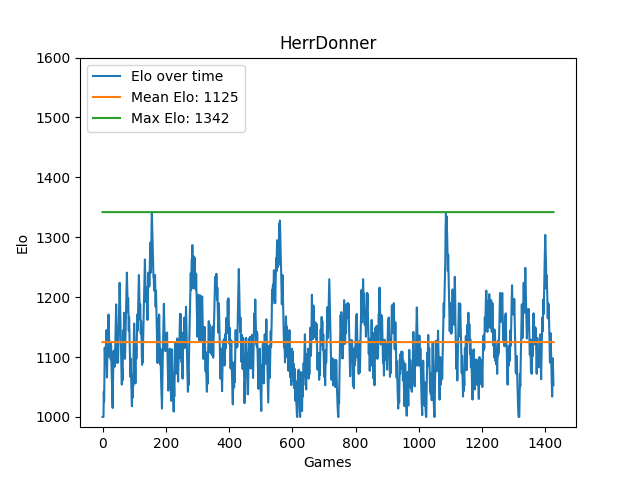
\includegraphics[width=1\linewidth]{images/Donner-Elo-Time.png}
      \captionof{figure}{Elo HerrDonner}
      \label{fig:donner-elo}
    \end{minipage}%
    \begin{minipage}{.5\textwidth}
      \centering
      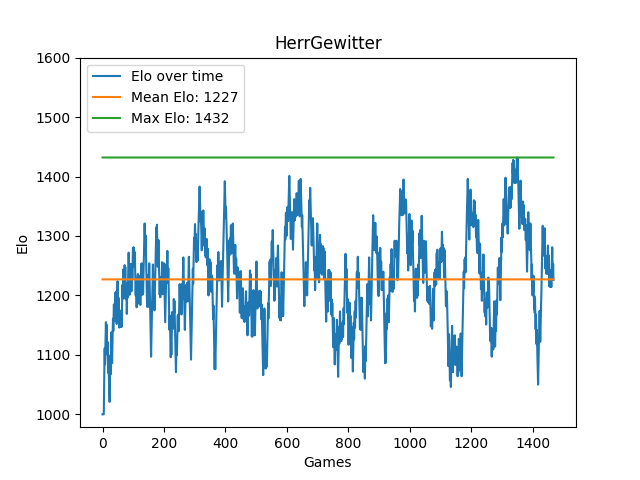
\includegraphics[width=1\linewidth]{images/Gewitter-Elo-Time.png}
      \captionof{figure}{Elo HerrGewitter}
      \label{fig:gewitter-elo}
    \end{minipage}
\end{figure}
    
\begin{figure}[h]
	\centering
	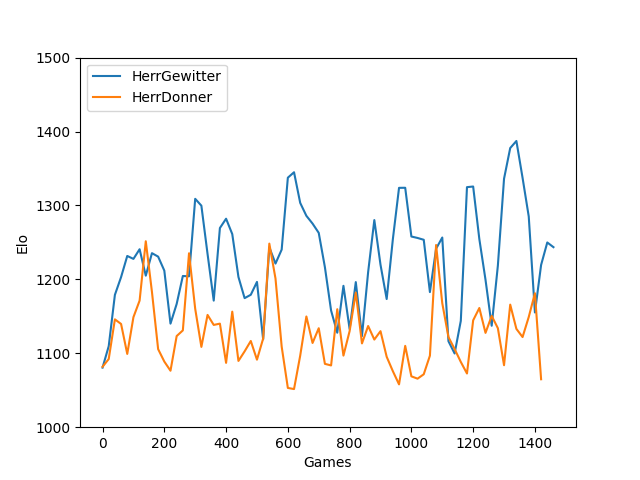
\includegraphics[width=0.7\textwidth]{images/Smoothed-Elo-Time.png}
	\caption{Smoothed Elo}
	\label{fig:elo-smoothed}
\end{figure}
 